\clearpage
\subsection{Majority-class chance level}
\label{app:majority_chance}

The above-chance filter of Appendix~\ref{app:chance-threshold} compares every run with uniform guessing. When the gold answers of a task are unbalanced, a model that always picks the most frequent gold option scores that option's share of the items, which can exceed $1/m_b$. We test how much the filter depends on this choice. For every accuracy task, we read the gold option position of each evaluated item and compute the majority baseline, the accuracy of always choosing the most frequent position. We then rerun the filter on the same runs and with the same Wilson rule, taking as chance level the larger of the uniform level and the majority baseline. The rest of the paper keeps the uniform filter.

The majority baseline is attainable only where a position means the same answer on every item, as with lettered options or a fixed set of labels such as yes and no. On cloze tasks whose answers change from item to item, the model scores each answer by its log-likelihood and never sees its position. On these tasks, the majority baseline reflects how the dataset orders its answers. MultiBLiMP always lists the grammatical sentence first and TruthfulQA its true answers first, so their majority baseline is 1.0. We therefore also report the filter with the majority level applied to the labelled tasks only.

Figure~\ref{fig:app_rq00_majority_chance} shows the result. Applied to every task, the majority level removes 45\% of the passing (task, size) cells of the trained tasks. Almost all of the removed cells belong to cloze tasks with item-specific answers, whose position skew no log-likelihood model can use. Applied to the labelled tasks only, it lowers the share of trained tasks above chance by 1.4 to 2.7 percentage points, depending on the size. It removes few tasks: the NoReC sentiment tasks, CulturalBench-easy (whose small answer keys are unbalanced), PAWS-X, BBH (MCQ), BLEnD, and the letter-format Belebele, Global-MMLU and INCLUDE tasks that the uniform filter only just passed. Under either majority filter, the decision accuracy of a proxy against the 1.7B reference on accuracy moves by at most 0.006. When only the labelled tasks change, the share of tasks with predictable scaling along both model size and training is 76\%, against 74\% under the uniform filter.

\begin{figure*}[p]
\centering
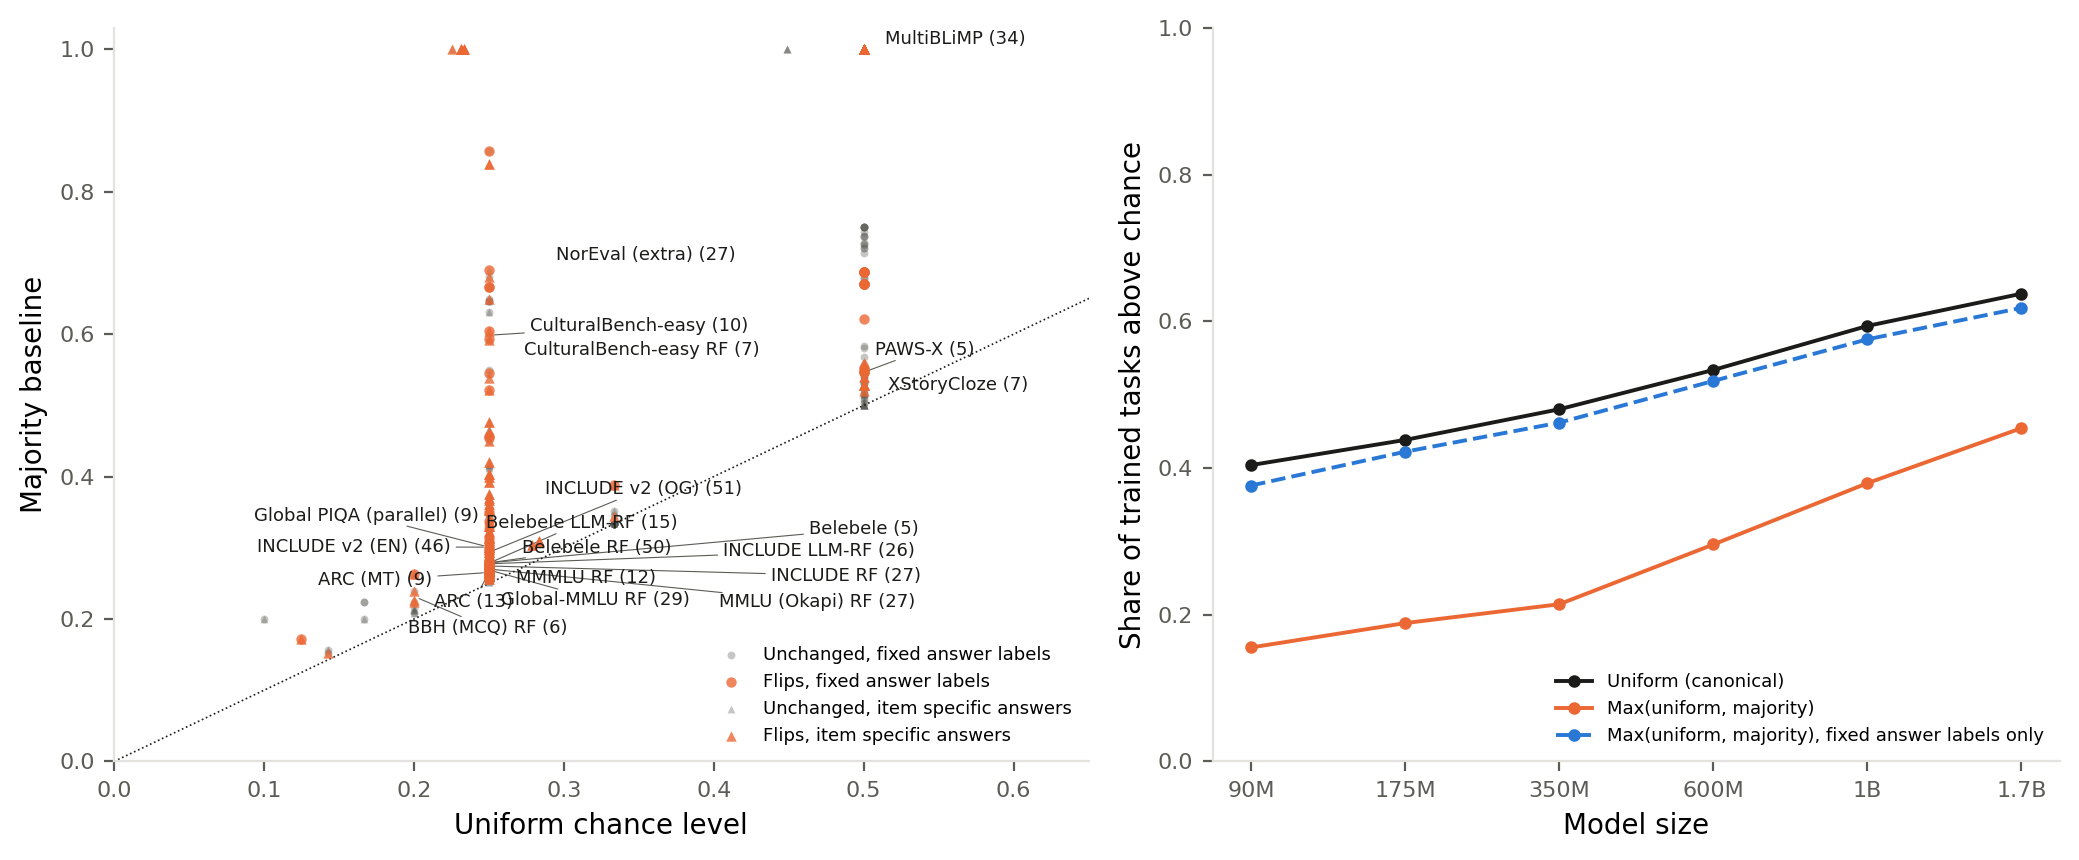
\includegraphics[width=\textwidth,height=0.8\textheight,keepaspectratio]{figures/app_rq00_majority_chance.png}
% source: src/signal-and-noise/analysis/rq00_gate_and_curves/majority_chance/majority_chance_paper.png
\caption{\textbf{A majority-class chance level removes passes mainly through answer order, which log-likelihood scoring cannot exploit.} The majority baseline of a task is the accuracy of always choosing its most frequent gold option position, read from the evaluated items. (a) Uniform chance against the majority baseline for the 933 trained tasks with a chance level. Orange marks the 447 tasks above chance at some size under the uniform level and at chance there under the larger of the two, with a benchmark label where a benchmark has at least five such tasks. Circles are tasks whose answer positions carry the same label on every item (a letter or a yes or no answer), where a model with a constant preference can reach the majority baseline. Triangles are tasks whose answers change per item. (b) Trained tasks above chance per size under the uniform level, under the majority level, and under the majority level applied to the labelled tasks only. Of the 933 trained tasks, 377 are above chance at 90M and 595 at 1.7B under the uniform level, 145 and 424 under the majority level, and 351 and 577 when only the labelled tasks change. Of the flipped tasks, 42 are labelled. Seed-1904 runs of every language setting, ladder and data build, with the Wilson rule of Appendix~\ref{app:chance-threshold}.}
\label{fig:app_rq00_majority_chance}
\end{figure*}

